\documentclass[10pt]{article}
\usepackage[a4paper,margin=18mm]{geometry}
\usepackage{amsmath,amssymb,booktabs,array,enumitem}
\usepackage[T1]{fontenc}\usepackage{lmodern}
\usepackage{tikz}\usetikzlibrary{shapes.gates.logic.US,positioning,arrows.meta,patterns,calc}
\usepackage[hidelinks]{hyperref}
\setlength{\parindent}{0pt}\setlength{\parskip}{4pt}
\setlength{\emergencystretch}{2em}
\newcommand{\VDD}{V_{DD}}
\newcommand{\mos}[4]{\begin{scope}[shift={(#1,#2)}]
\draw (0,.24)--(0,-.24);\draw (0,.20)--(.25,.20)--(.25,.5);
\draw (0,-.20)--(.25,-.20)--(.25,-.5);\draw (-.16,.23)--(-.16,-.23);
\ifnum#4=1\draw (-.26,0) circle (.06);\draw (-.75,0)--(-.32,0);\else\draw (-.75,0)--(-.16,0);\fi
\node[anchor=east,font=\scriptsize] at (-.76,0) {$#3$};\end{scope}}
\newcommand{\ground}[2]{\draw (#1,#2)--(#1,{#2-.12});\draw ({#1-.17},{#2-.12})--({#1+.17},{#2-.12});\draw ({#1-.11},{#2-.20})--({#1+.11},{#2-.20});}
\newcommand{\rail}[3]{\draw (#1,#2)--(#1,{#2+.14});\node[above,font=\scriptsize] at (#1,{#2+.14}) {$#3$};}

\newcommand{\hmos}[4]{\begin{scope}[shift={(#1,#2)}]
\draw(-.24,0)--(.24,0);\draw(-.2,0)--(-.2,-.25)--(-.5,-.25);\draw(.2,0)--(.2,-.25)--(.5,-.25);
\draw(-.23,.16)--(.23,.16);
\ifnum#4=1\draw(0,.26)circle(.06);\draw(0,.32)--(0,.75);\else\draw(0,.16)--(0,.75);\fi
\node[below,font=\scriptsize]at(0,-.32){#3};\end{scope}}
\begin{document}
\begin{center}{\large\bfseries EE3032 Introduction to VLSI Design -- Final}\par Fall 2024\end{center}
\textbf{1. (45 points)} Answer the following questions.
\begin{enumerate}[label=(\alph*),leftmargin=7mm,itemsep=4pt]
\item List the components of dynamic power consumption of a dynamic logic gate. (6 points)
\item The power integrity (IR drop) of an IC is related to the design of power distribution network. List two approaches to improve the power integrity. (6 points)
\item Explain the latchup phenomenon. List a design approach which can alleviate the occurrence probability of latchup. (6 points)
\item Negative bias temperature instability (NBTI) is one of primary mechanisms for oxide wearout. Explain the principle of NBTI. (4 points)
\item List two design approaches for overcome the issue of hold time violation in a shift register. (6 points)
\item List two requirements for drawing the layout of a cell in the standard cell library. (4 points)
\item List two methods to reduce the power bounce and ground bounce occurring in the IO circuits. (4 points)
\item List two design methods for avoiding glitch power of a CMOS circuit. (4 points)
\item Design $f=\overline{x_1x_2+x_3}$ using differential pass transistor logic. Draw the transistor-level schematic diagram. (5 points)
\end{enumerate}
\textbf{2. (5 points)} If we want to design a 3-bit adder, we can use the carry generation function $c_{i+1}=p_i c_i+g_i$ for $i=0,1,2$ to generate the carries $c_1,c_2,c_3$ of the adder. Design a carry generation circuit with inputs $c_0,p_0,p_1,p_2,g_0,g_1,g_2$ for a 3-bit adder using multioutput domino logic. Draw the transistor-level schematic diagram.

\textbf{3. (15 points)} Fig. 1 shows a simple circuit with three gates. Complete the following questions.
\begin{enumerate}[label=(\alph*),leftmargin=7mm,itemsep=4pt]
\item Can the circuit be operated correctly? Explain your answer. If your answer is ``no'', modify the circuit such that it can be operated correctly. (5 points)
\item Assume that each transistor of the (modified) circuit has the following drain and gate capacitance: $C_d=0.1\,\mathrm{fF}$, $C_g=1\,\mathrm{fF}$; and the parasitic capacitance of the node $x$ and $y$ are $1.3\,\mathrm{fF}$ and $1.1\,\mathrm{fF}$, respectively. Let the switching voltage of all the gates in the (modified) circuit be $V_{DD}/2$. Can the circuit be operated correctly? Explain your answer. (5 points)
\item The clock period of the (modified) circuit cannot be prolonged casually. Why? Modify the circuit such that its clock period can be prolonged casually. Draw the transistor schematic diagram. (5 points)
\end{enumerate}
\begin{center}\begin{tikzpicture}[scale=.82,font=\small]
\mos{2}{4}{\phi}{1}\rail{2.25}{4.5}{V_{DD}}
\draw(.25,3.5)--(3.25,3.5);\fill(2.25,3.5)circle(1.5pt);\node[above]at(1.3,3.5){$Z$};
\mos{0}{3}{A}{0}\mos{0}{2}{B}{0}\mos{3}{3}{C}{0}\mos{2}{2}{A}{0}\mos{4}{2}{B}{0}
\draw(2.25,2.5)--(4.25,2.5);\fill(3.25,2.5)circle(1.5pt);\node[above]at(3.7,2.5){$y$};\node[right]at(.25,2.5){$x$};
\draw(.25,1.5)--(4.25,1.5);\mos{2}{1}{\phi}{0}\ground{2.25}{.5}
\mos{7}{3.8}{\bar\phi}{1}\rail{7.25}{4.3}{V_{DD}}\mos{7}{2.5}{Z}{0}\draw(7.25,3)--(7.25,3.3);\draw(7.25,3.15)--(8.25,3.15)node[pos=.55,above]{$\bar Y$};
\mos{7}{1.5}{\bar\phi}{0}\ground{7.25}{1}
\mos{10}{4}{\bar\phi}{1}\rail{10.25}{4.5}{V_{DD}}\mos{10}{3}{Z}{1}\mos{10}{1.8}{\bar\phi}{0}\draw(10.25,2.3)--(10.25,2.5)--(11.1,2.5)node[right]{$X$};\ground{10.25}{1.3}
\draw(2.25,3.5)--(5.75,3.5);\draw(5.75,2.5)--(5.75,3.5);\draw(6.0,1.5)--(6.0,3.8)--(6.25,3.8);\draw(6.0,1.5)--(6.25,1.5);\draw(5.75,2.5)--(6.25,2.5);\fill(5.75,3.5)circle(1.5pt);\draw(5.75,3.5)--(9,3.5)--(9,3)--(9.25,3);
\end{tikzpicture}\end{center}\begin{center}\small Figure 1: A simple circuit.\end{center}
\newpage
\textbf{4. (11 points)} Fig. 2(a) shows a Schmitt trigger circuit. If we apply an input signal as shown in the left figure to the Schmitt trigger circuit, the output signal will be as the right figure shows. Assume that $\mu_n=2\mu_p$, the drain parasitic capacitance of all the transistors can be ignored, and the simple RC delay model is used to estimate the delay. Complete the following questions.
\begin{enumerate}[label=(\alph*),leftmargin=7mm,itemsep=4pt]
\item Let $V_{tn}=|V_{tp}|=0.2\,\mathrm V$ and $V_{DD}=1.5\,\mathrm V$. If the size of N1 is $160\,\mathrm{nm}/40\,\mathrm{nm}$, determine the sizes of the transistors N2, N3, P1, P2 and P3 such that $t_r=t_f=3RC$, where the turn-on resistance and gate capacitance of N1 is $R$ and $C$. All the transistors should have the same channel length. (5 points)
\item Fig. 2(b) shows Schmitt trigger circuit (STC) with controllable hysteresis voltage ($V_H$) by controlling the switches (sw). If the switches are turned on, is the noise tolerance capability of the STC increased or decreased? Is the short-circuit power of STC increased or decreased? Explain your answers. (6 points)
\end{enumerate}
\begin{center}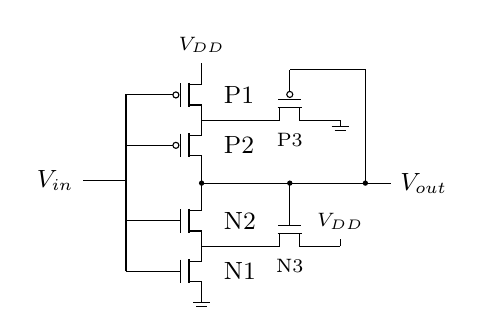
\begin{tikzpicture}[scale=0.64,font=\small]
\mos{1}{5}{}{1}\mos{1}{4}{}{1}\mos{1}{2.5}{}{0}\mos{1}{1.5}{}{0}
\rail{1.25}{5.5}{V_{DD}}\ground{1.25}{1}\draw(1.25,3)--(1.25,3.5);\draw(1.25,3.25)--(5.0,3.25)node[right]{$V_{out}$};\fill(1.25,3.25)circle(1.5pt);
\draw(-.25,1.5)--(-.25,5)--(.25,5);\draw(-.25,4)--(.25,4);\draw(-.25,2.5)--(.25,2.5);\draw(-.25,1.5)--(.25,1.5);\draw(-1.1,3.3)--(-.25,3.3)node[pos=0,left]{$V_{in}$};
\node[right]at(1.5,5){P1};\node[right]at(1.5,4){P2};\node[right]at(1.5,2.5){N2};\node[right]at(1.5,1.5){N1};
\hmos{3}{4.75}{P3}{1}\draw(1.25,4.5)--(2.5,4.5);\draw(3.5,4.5)--(4,4.5);\ground{4}{4.5}
\hmos{3}{2.25}{N3}{0}\draw(1.25,2)--(2.5,2);\draw(3.5,2)--(4,2);\rail{4}{2}{V_{DD}}
\draw(3,3)--(3,3.25);\fill(3,3.25)circle(1.5pt);\draw(3,5.5)--(4.5,5.5)--(4.5,3.25);\fill(4.5,3.25)circle(1.5pt);
\end{tikzpicture}\qquad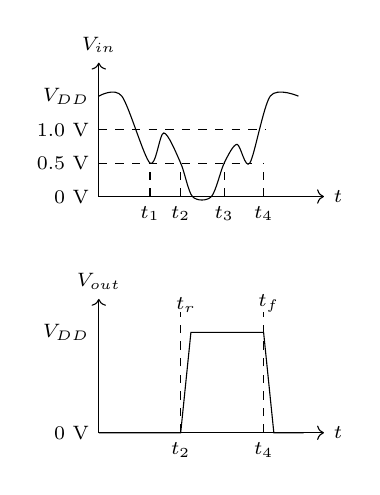
\begin{tikzpicture}[x=.65cm,y=.85cm,font=\scriptsize]
\draw[->](0,0)--(4.4,0)node[right]{$t$};\draw[->](0,0)--(0,2.0)node[above]{$V_{in}$};
\draw plot[smooth]coordinates{(0,1.5)(.45,1.5)(1,.5)(1.27,.95)(1.6,.5)(1.83,0)(2.2,0)(2.45,.5)(2.7,.78)(2.95,.5)(3.35,1.5)(3.9,1.5)};
\draw[dashed](0,1)--(3.25,1);\draw[dashed](0,.5)--(3.0,.5);\node[left]at(0,1.5){$V_{DD}$};\node[left]at(0,1){1.0 V};\node[left]at(0,.5){0.5 V};\node[left]at(0,0){0 V};
\foreach\x/\l in {1/1,1.6/2,2.45/3,3.22/4}{\draw[dashed](\x,0)--(\x,.5);\node[below]at(\x,0){$t_\l$};}
\begin{scope}[yshift=-3cm]
\draw[->](0,0)--(4.4,0)node[right]{$t$};\draw[->](0,0)--(0,2)node[above]{$V_{out}$};\node[left]at(0,1.5){$V_{DD}$};\node[left]at(0,0){0 V};
\draw(0,0)--(1.6,0)--(1.8,1.5)--(3.22,1.5)--(3.42,0)--(4.0,0);\draw[dashed](1.6,0)--(1.6,1.8);\draw[dashed](3.22,0)--(3.22,1.8);\node[above]at(1.7,1.65){$t_r$};\node[above]at(3.32,1.65){$t_f$};\node[below]at(1.6,0){$t_2$};\node[below]at(3.22,0){$t_4$};
\end{scope}\end{tikzpicture}\par (a)\end{center}
\begin{center}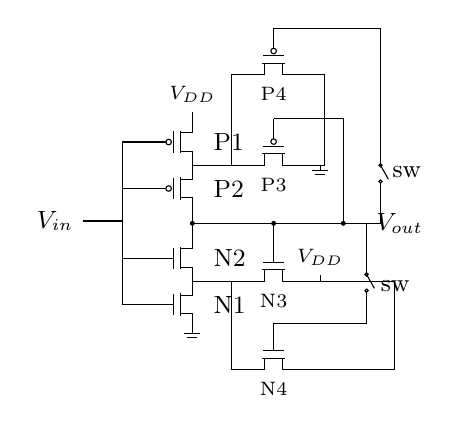
\begin{tikzpicture}[scale=0.59,font=\small]
\mos{1}{5}{}{1}\mos{1}{4}{}{1}\mos{1}{2.5}{}{0}\mos{1}{1.5}{}{0}
\rail{1.25}{5.5}{V_{DD}}\ground{1.25}{1}\draw(1.25,3)--(1.25,3.5);\draw(1.25,3.25)--(5.0,3.25)node[right]{$V_{out}$};\fill(1.25,3.25)circle(1.5pt);
\draw(-.25,1.5)--(-.25,5)--(.25,5);\draw(-.25,4)--(.25,4);\draw(-.25,2.5)--(.25,2.5);\draw(-.25,1.5)--(.25,1.5);\draw(-1.1,3.3)--(-.25,3.3)node[pos=0,left]{$V_{in}$};
\node[right]at(1.5,5){P1};\node[right]at(1.5,4){P2};\node[right]at(1.5,2.5){N2};\node[right]at(1.5,1.5){N1};
\hmos{3}{4.75}{P3}{1}\draw(1.25,4.5)--(2.5,4.5);\draw(3.5,4.5)--(4,4.5);\ground{4}{4.5}
\hmos{3}{2.25}{N3}{0}\draw(1.25,2)--(2.5,2);\draw(3.5,2)--(4,2);\rail{4}{2}{V_{DD}}
\draw(3,3)--(3,3.25);\fill(3,3.25)circle(1.5pt);\draw(3,5.5)--(4.5,5.5)--(4.5,3.25);\fill(4.5,3.25)circle(1.5pt);
\hmos{3}{6.7}{P4}{1}\draw(1.25,4.5)--(2.1,4.5)--(2.1,6.45)--(2.5,6.45);\draw(3.5,6.45)--(4.1,6.45)--(4.1,4.5)--(4,4.5);
\hmos{3}{.35}{N4}{0}\draw(1.25,2)--(2.1,2)--(2.1,.1)--(2.5,.1);\draw(3.5,.1)--(5.6,.1)--(5.6,2)--(4,2);
\draw(3,7.45)--(5.3,7.45)--(5.3,4.5);\draw(5.3,4.15)--(5.3,3.25)--(4.5,3.25);\draw(5.3,4.5)--(5.47,4.2);\draw(5.3,4.5)circle(.035);\draw(5.3,4.15)circle(.035);\node[right]at(5.35,4.35){sw};
\draw(3,1.1)--(5.0,1.1)--(5.0,1.8);\draw(5.0,2.15)--(5.0,3.25);\draw(5.0,2.15)--(5.17,1.85);\draw(5.0,1.8)circle(.035);\draw(5.0,2.15)circle(.035);\node[right]at(5.1,1.9){sw};
\end{tikzpicture}\par (b)\end{center}
\begin{center}\small Figure 2: (a) A CMOS Schmitt trigger circuit (b) A STC with controllable hysteresis voltage.\end{center}
\newpage
\textbf{5. (10 points)} Draw the transistor-level schematic diagram of the symbolic layout shown in Fig. 3(a).
% Normalized topological geometry: 7 crossings/row, 14physical MOS.
\usetikzlibrary{patterns}
\begin{center}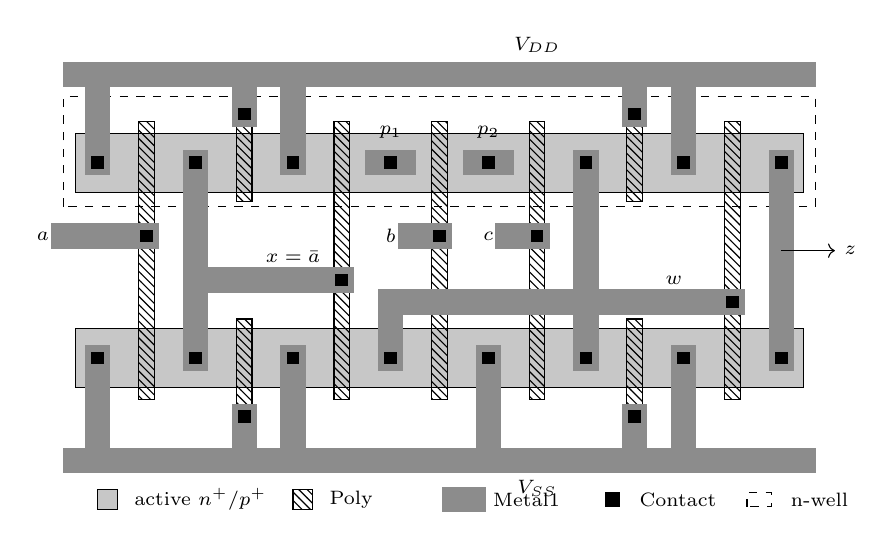
\begin{tikzpicture}[x=.62cm,y=.62cm,font=\scriptsize]
\tikzset{mone/.style={draw=black!45,line width=.32cm,line cap=rect},poly/.style={draw,pattern=north west lines}}
% Continuous active diffusion strips and upper n-well.
\filldraw[fill=black!22](-.45,4) rectangle(14.45,5.2);
\filldraw[fill=black!22](-.45,0) rectangle(14.45,1.2);
\draw[dashed](-.7,3.7)rectangle(14.7,5.95);
% Functional polys: a, x, b, c, w. Two split isolation columns: 2 and6.
\foreach \g in {1,5,7,9,13}{\filldraw[poly](\g-.16,-.25)rectangle(\g+.16,5.45);}
\foreach \g in {3,11}{\filldraw[poly](\g-.16,3.8)rectangle(\g+.16,5.65);\filldraw[poly](\g-.16,-.7)rectangle(\g+.16,1.4);}
% Metal1 rail distribution and contact branches.
\draw[mone](-.45,6.4)--(14.45,6.4);\node[above]at(9,6.65){$V_{DD}$};
\draw[mone](-.45,-1.5)--(14.45,-1.5);\node[below]at(9,-1.7){$V_{SS}$};
\foreach \x in {0,4,12}{\draw[mone](\x,4.6)--(\x,6.4);\fill(\x-.13,4.47)rectangle(\x+.13,4.73);}
\foreach \x in {0,4,8,12}{\draw[mone](\x,.6)--(\x,-1.5);\fill(\x-.13,.47)rectangle(\x+.13,.73);}
% Left inverter drain strap x, feeding column3 via metal/poly contact.
\draw[mone](2,.6)--(2,4.6);\fill(1.87,.47)rectangle(2.13,.73);\fill(1.87,4.47)rectangle(2.13,4.73);
\draw[mone](2,2.2)--(5,2.2);\fill(4.87,2.07)rectangle(5.13,2.33);\node[above]at(4,2.35){$x=\bar a$};
% Series-PMOS internal local contact/metal patches: p1,p2, not supply.
\foreach \x/\n in {6/p_1,8/p_2}{\draw[mone](\x-.27,4.6)--(\x+.27,4.6);\fill(\x-.13,4.47)rectangle(\x+.13,4.73);\node[above]at(\x,4.9){$\n$};}
% w joins PMOS segment5/6, NMOS3/4 and5/6, then drives column7.
\draw[mone](10,.6)--(10,4.6);\fill(9.87,.47)rectangle(10.13,.73);\fill(9.87,4.47)rectangle(10.13,4.73);
\draw[mone](6,.6)--(6,1.75)--(13,1.75);\draw[mone](10,1.75)--(13,1.75);
\fill(5.87,.47)rectangle(6.13,.73);\fill(12.87,1.62)rectangle(13.13,1.88);\node[above]at(11.8,1.9){$w$};
% Right inverter drain strap, labeled output z.
\draw[mone](14,.6)--(14,4.6);\fill(13.87,.47)rectangle(14.13,.73);\fill(13.87,4.47)rectangle(14.13,4.73);
\draw[->](14,2.8)--(15.1,2.8)node[right]{$z$};
% Input metal/poly contacts; rail-tied isolation gate stubs.
\draw[mone](-.7,3.1)--(1,3.1);\fill(.87,2.97)rectangle(1.13,3.23);\node[left]at(-.8,3.1){$a$};
\draw[mone](6.4,3.1)--(7,3.1);\fill(6.87,2.97)rectangle(7.13,3.23);\node[left]at(6.3,3.1){$b$};
\draw[mone](8.4,3.1)--(9,3.1);\fill(8.87,2.97)rectangle(9.13,3.23);\node[left]at(8.3,3.1){$c$};
\foreach \g in {3,11}{\draw[mone](\g,5.6)--(\g,6.4);\fill(\g-.13,5.47)rectangle(\g+.13,5.73);\draw[mone](\g,-.6)--(\g,-1.5);\fill(\g-.13,-.73)rectangle(\g+.13,-.47);}
% Layer legend. A crossing without a black contact square is insulated.
\filldraw[fill=black!22](0,-2.5)rectangle(.4,-2.1);\node[right]at(.55,-2.3){active $n^+/p^+$};
\filldraw[poly](4,-2.5)rectangle(4.4,-2.1);\node[right]at(4.55,-2.3){Poly};
\draw[mone](7.3,-2.3)--(7.7,-2.3);\node[right]at(7.9,-2.3){Metal1};
\fill(10.4,-2.45)rectangle(10.7,-2.15);\node[right]at(10.9,-2.3){Contact};
\draw[dashed](13.3,-2.45)rectangle(13.8,-2.15);\node[right]at(14,-2.3){n-well};
\end{tikzpicture}\end{center}
\begin{center}\small Figure 3(a): Symbolic layout.\end{center}
% Original gates retained: XOR, twoNANDs, finalNOR, lowerXOR.
\usetikzlibrary{shapes.gates.logic.US}
\begin{center}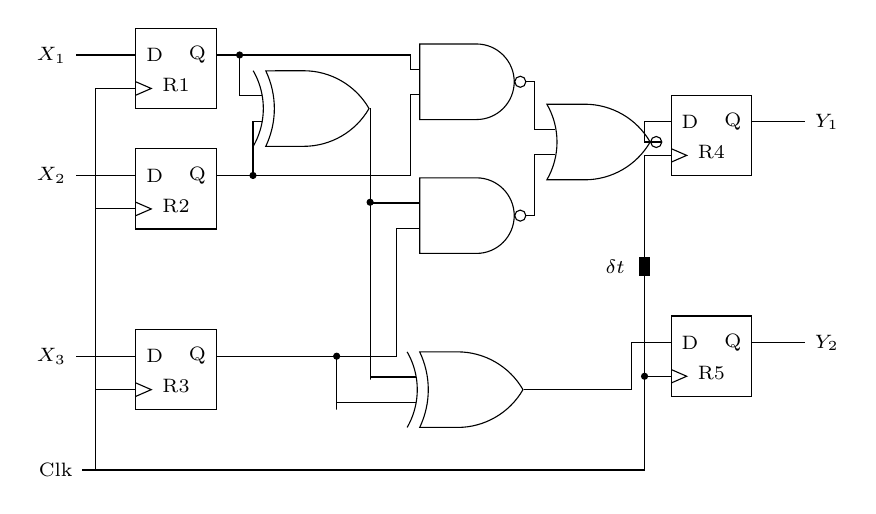
\begin{tikzpicture}[x=.85cm,y=.85cm,font=\scriptsize]
\foreach \n/\x/\y in {1/0/3,2/0/1.2,3/0/-1.5,4/8/2,5/8/-1.3}{
\draw(\x-.6,\y-.6)rectangle(\x+.6,\y+.6);
\node at(\x-.32,\y+.2){D};\node at(\x+.32,\y+.2){Q};\node at(\x,\y-.25){R\n};
\draw(\x-.6,\y-.4)--(\x-.37,\y-.3)--(\x-.6,\y-.2);
\coordinate(Q\n)at(\x+.6,\y+.2);\coordinate(D\n)at(\x-.6,\y+.2);\coordinate(K\n)at(\x-.6,\y-.3);
}
\foreach \n in {1,2,3}{\draw(D\n)--++(-.9,0)node[left]{$X_\n$};}
\draw(Q4)--++(.8,0)node[right]{$Y_1$};\draw(Q5)--++(.8,0)node[right]{$Y_2$};
\node[xor gate US,draw,logic gate inputs=nn,logic gate input sep=.32cm] (GX)at(2.0,2.4){};
\node[nand gate US,draw,logic gate inputs=nn,logic gate input sep=.32cm] (GU)at(4.3,2.8){};
\node[nand gate US,draw,logic gate inputs=nn,logic gate input sep=.32cm] (GV)at(4.3,.8){};
\node[nor gate US,draw,logic gate inputs=nn,logic gate input sep=.32cm] (GO)at(6.2,1.9){};
\node[xor gate US,draw,logic gate inputs=nn,logic gate input sep=.32cm] (GY)at(4.3,-1.8){};
\draw(Q1)--(.95,3.2)|-(GX.input 1);\fill(.95,3.2)circle(1.3pt);\draw(.95,3.2)--(3.5,3.2)|-(GU.input 1);
\draw(Q2)--(1.15,1.4)|-(GX.input 2);\fill(1.15,1.4)circle(1.3pt);\draw(1.15,1.4)--(3.5,1.4)|-(GU.input 2);
\draw(GX.output)--(2.9,2.4)--(2.9,-1.65)|-(GY.input 1);\fill(2.9,1.0)circle(1.3pt);\draw(2.9,1.0)|-(GV.input 1);
\draw(Q3)--(2.4,-1.3)--(3.3,-1.3)|-(GV.input 2);\fill(2.4,-1.3)circle(1.3pt);\draw(2.4,-1.3)--(2.4,-2.1)|-(GY.input 2);
\draw(GU.output)--(5.35,2.8)|-(GO.input 1);\draw(GV.output)--(5.35,.8)|-(GO.input 2);
\draw(GO.output)--(7,1.9)|-(D4);\draw(GY.output)--(6.8,-1.8)|-(D5);
% One common clock source. R5 taps before R4's physical delta-t element.
\draw(-1.4,-3)node[left]{Clk}--(7.0,-3)--(7.0,-.10);
\draw(-1.2,-3)--(-1.2,2.7);\foreach \n in {1,2,3}{\draw(-1.2,0 |- K\n)--(K\n);}
\draw(7,-1.6)--(K5);\fill(7,-1.6)circle(1.3pt);
\filldraw(6.92,-.10)rectangle(7.08,.18);\node[left]at(6.85,.04){$\delta t$};
\draw(7,.18)--(7,1.7)--(K4);
\end{tikzpicture}\end{center}
\begin{center}\small Figure 3(b): A sequential circuit.\end{center}
\textbf{6. (24 points)} Fig. 3(b) shows a sequential circuit. Assume that the clock-to-Q propagation delay ($t_{pcq}$), the clock-to-Q contamination delay ($t_{ccq}$), the setup time ($t_{setup}$), and the hold time ($t_{hold}$) of the registers are $0.2\,\mathrm{ns}$, $0.1\,\mathrm{ns}$, $0.2\,\mathrm{ns}$, and $0.2\,\mathrm{ns}$, respectively. Also, $\delta t=0.6\,\mathrm{ns}$, $t_{NAND}=0.5\,\mathrm{ns}$, $t_{NOR}=0.5\,\mathrm{ns}$, and $t_{XOR}=1\,\mathrm{ns}$. Complete the following questions.
\begin{enumerate}[label=(\alph*),leftmargin=7mm,itemsep=4pt]
\item Determine the maximum operation frequency of the circuit. (5 points)
\item Assume that the delay of an inverter is $0.3\,\mathrm{ns}$. Redesign the clock tree by doing buffer insertion such that the maximum operation frequency can be boosted to 400 MHz. Draw the clock tree including the registers. (5 points)
\item Design the combinational circuit using NP-domino logic style. Draw the transistor-level schematic diagram. (10 points)
\item In the two registers, R4 and R5, which register has higher soft error rate? Explain your answer. (4 points)
\end{enumerate}
\vfill\small Li, EE, NCU. Typeset transcription; all figures are editable vectors. The middle clock overbar touches a wire in the scan; its phase readings are discussed in the solution. The original printed point allocations sum to 110; they are retained without rescaling. Original annotations and photo perspective are excluded.
\end{document}
